\documentclass[14pt,utf8,hyperref={pdfpagelabels=false}]{beamer}
\usepackage{etex}
\usepackage{media9}

\usepackage[utf8]{inputenc} % hyperref broken with utf8x
\usepackage[C40,T1]{fontenc}

\usepackage{graphicx}
\usepackage{array}
\usepackage{multirow}

\usepackage[francais]{babel}

\usepackage{algorithmic, algorithm}

\usepackage{tikz, pgfplots}
\usepackage{tikz-qtree}

\newcommand{\umltextcolor}{ThoughfulBrick}
\newcommand{\umldrawcolor}{Thoughtless}
\newcommand{\umlfillcolor}{ThoughtBySome}
\usepackage{pgf-umlcd}

%\reserveinserts{28}
%\usepackage{pgfpages}
%\setbeameroption{show notes on second screen}


\usetikzlibrary{shapes.arrows,chains,positioning,%
  matrix,patterns,shapes,shapes.multipart,positioning,arrows}
%\tikzexternalize

\tikzstyle{every picture}+=[remember picture]
\tikzstyle{na} = [baseline=-.5ex]

\tikzstyle{state}=[rectangle,
  color=structure.fg,
  fill=ThoughtBySome,
  inner sep=0.2cm,
  rounded corners=2mm]

\tikzstyle{mathbox} = [inner sep=0pt, anchor=base,%
  node distance=0pt, column sep=0em, thick]

\tikzset{
  template parameter/.style={
        append after command={
            node [draw, densely dashed, umlcolor, font=\ttfamily]
                at (\tikzlastnode.north east)
                {#1}
        }
    }
}

\tikzset{onslide/.code args={<#1>#2}{%
  \only<#1>{\pgfkeysalso{#2}}
}}

\newcommand{\tikzplaceholder}[1]{%
  \begingroup\shorthandoff{;}\tikz[na] \node[coordinate] (#1) {};\endgroup}

\newcommand{\blueoverlay}[2]{%
  \tikz[baseline]{ \node[fill=blue!20,anchor=base,rounded corners=2pt] (#1) {$#2$}; }}

\usetheme{moulardthesis}

\DeclareUnicodeCharacter{00A0}{~}

\title{Optimisation numérique\\
  Exécution~de~trajectoires référencées capteurs}
\author{Thomas Moulard}
\date{Lundi 17 septembre 2012}


% Setup pdf meta-data.
\hypersetup{
pdfauthor = {Thomas Moulard},
pdftitle = {Optimisation num\'erique pour la robotique%
 et ex\'ecution de trajectoires r\'ef\'erenc\'ees capteurs},
pdfsubject = {Optimisation num\'erique pour la robotique%
 et ex\'ecution de trajectoires r\'ef\'erenc\'ees capteurs},
pdfkeywords = {optimisation numérique, typage, type,%
robotique, humano\"ide},
pdfcreator = {Thomas Moulard},
pdfproducer = {Thomas Moulard}
}


\begin{document}

{
  \usebackgroundtemplate{%
    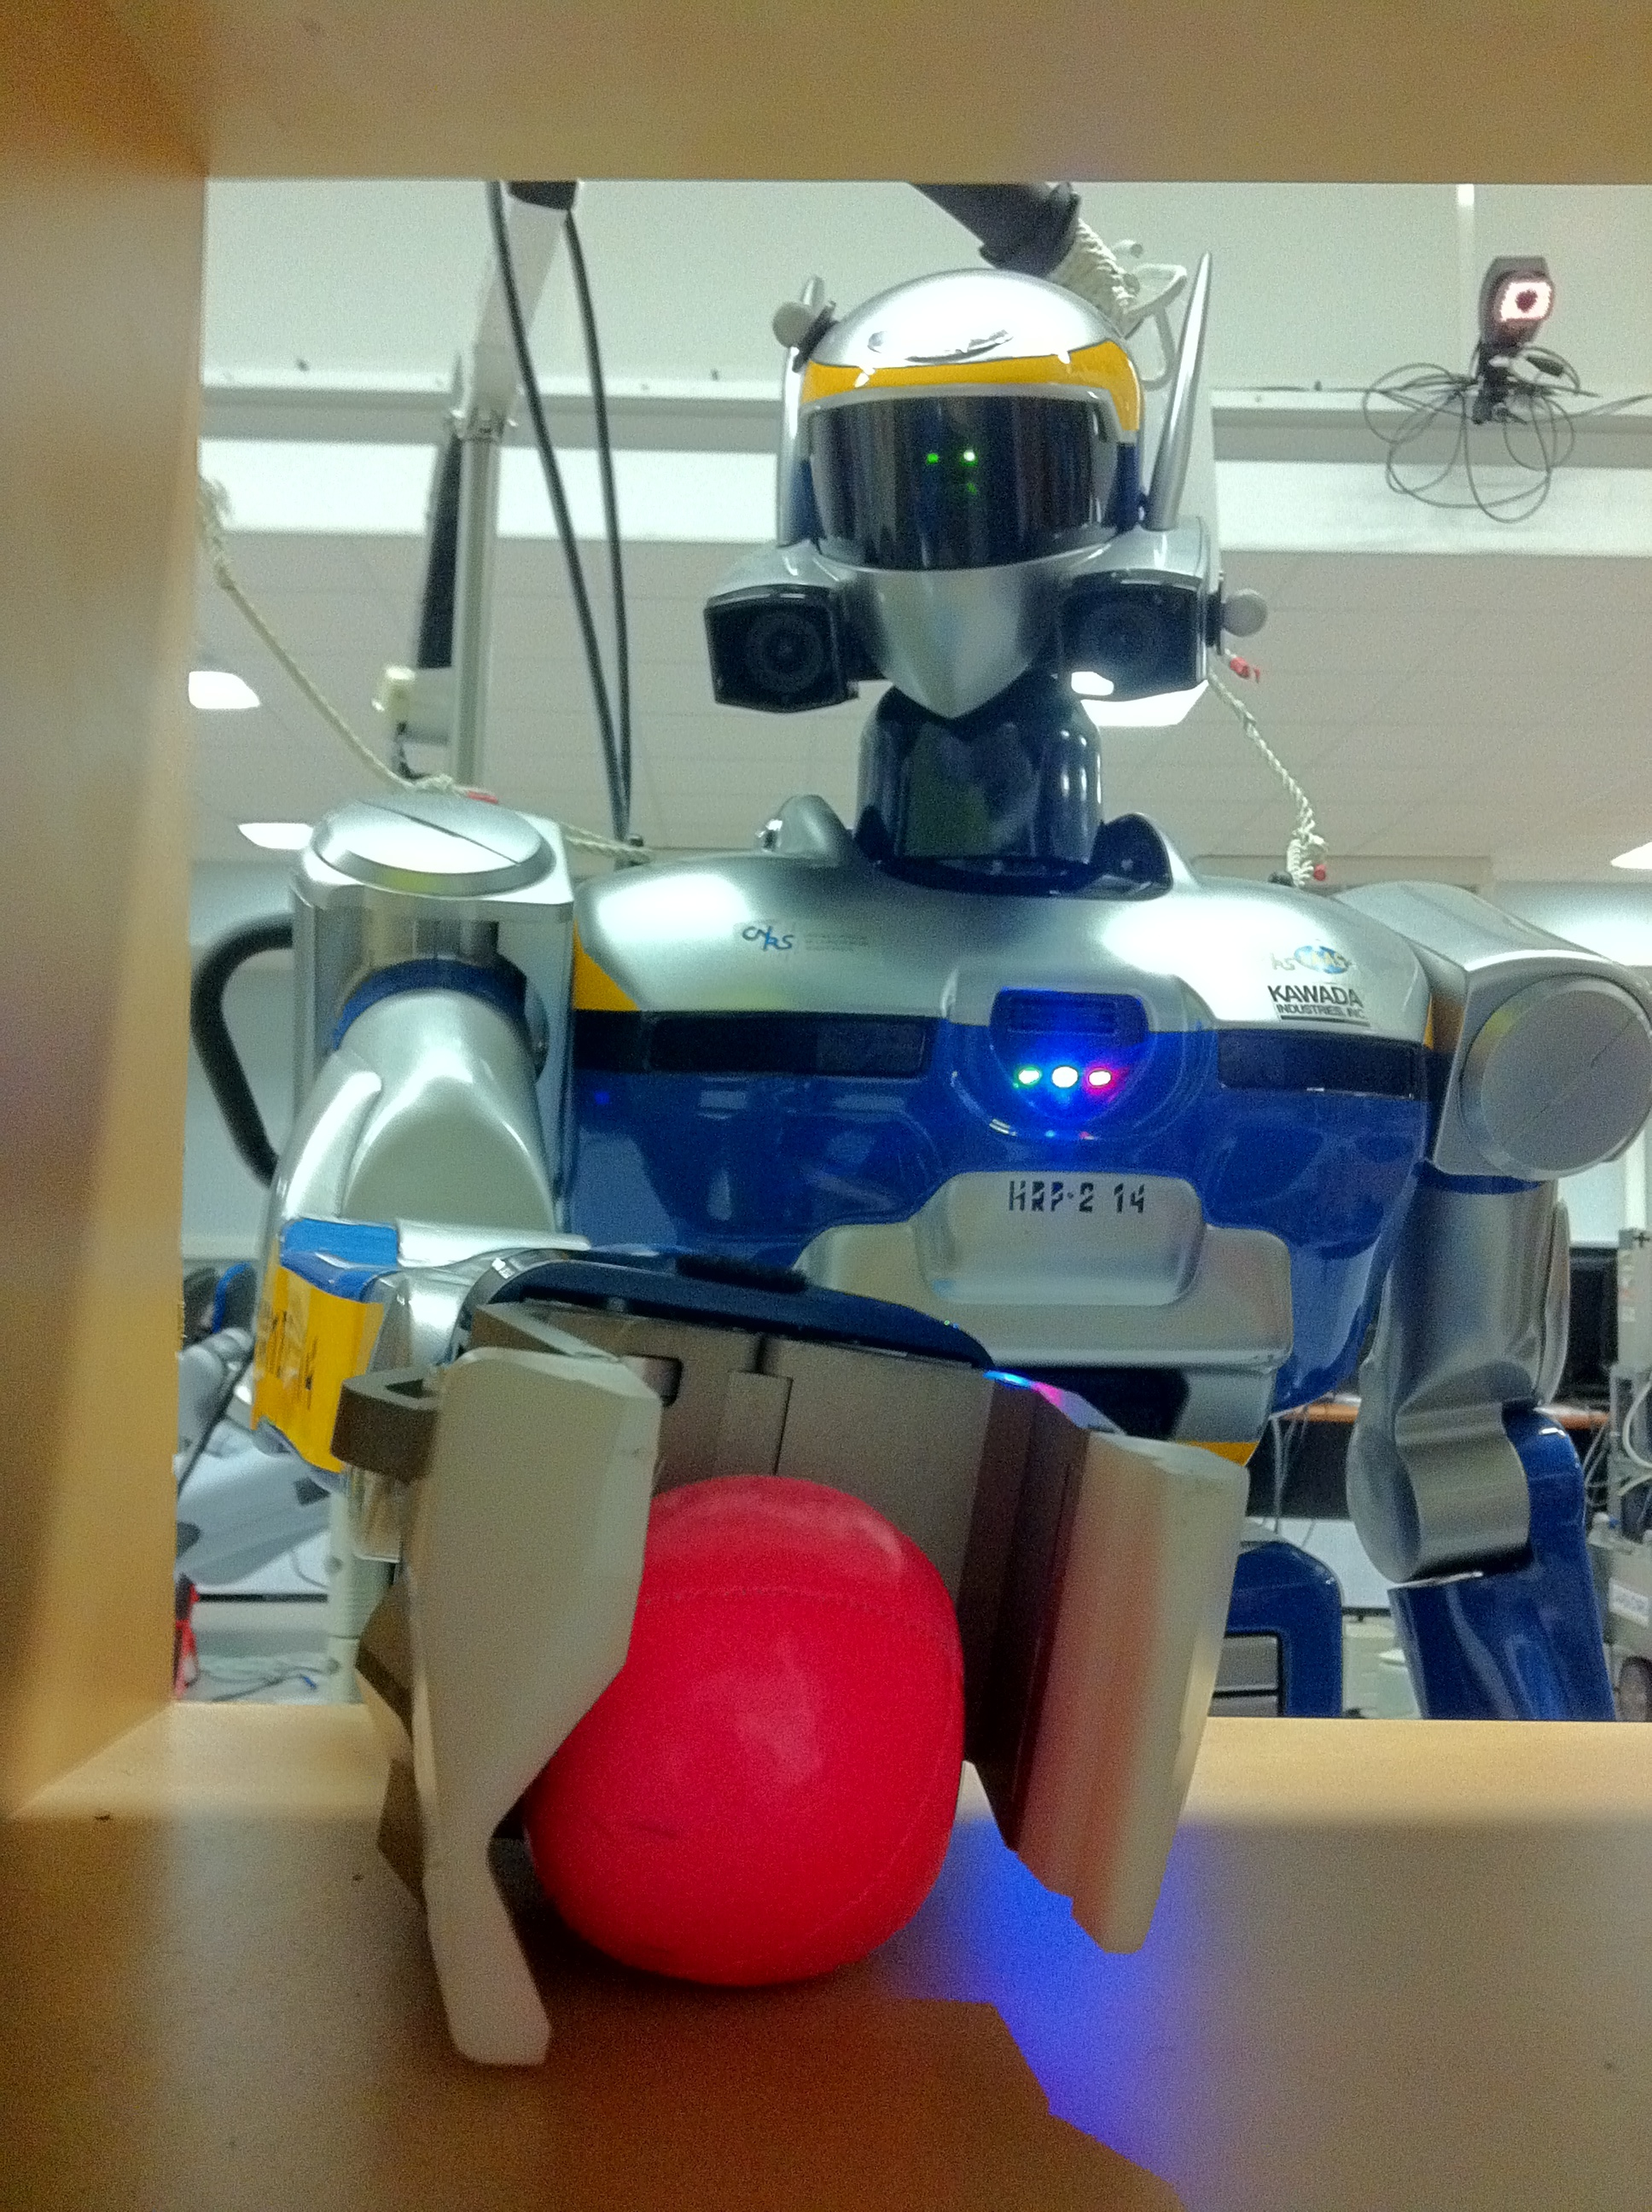
\includegraphics[width=\paperwidth,height=\paperheight]{%
      src/slides/demo1.jpg}}
  \begin{frame}[plain]
    \titlepage
    \note[item]{Remercier les rapporteurs, le jury}
  \end{frame}
}

%\maxFrameImage{src/slides/demo1.jpg}
%\maxFrameImage{src/slides/demo2.jpg}

% Introduction
% Animated scheme introducing contributions.
\begin{frame}[label=contrib]
  \note[item]{Architecture P-D-A}
  \note[item]{Perception: environnement, capteurs}
  \note[item]{Décision: résolution de l'objectif, planification}
  \note[item]{Action: commande des actioneurs}
  \note[item]{Contributions diverses pour les robots humanoïdes}
  \note[item]{RobOptim: représentation info des pb optim}
  \note[item]{Correction de trajectoire: %
    rebouclage capteur de la partie action}
  \note[item]{Primitives de mouvement: résultats préliminaires. %
    Planification de tâche, intégration capteurs dans la planificapteurs}
  %
  \begin{changemargin}{-1cm}{-1cm}
    \begin{center}
      \tikzstyle{normalPath} = [line width=.7mm, color=black!50, -latex]

      \begin{tikzpicture}[
          auto,
          state/.style={
            rectangle,
            minimum size=6mm
          }]

        \uncover<1->{
          \node (perception) [state] {%
            
\includegraphics[height=3cm]{%
              src/slides/perception.pdf}};
        }

        \uncover<1>{
          \node (perception-description)
                [state, right=of perception, yshift=-6mm, xshift=-6mm]
                {\textbf{Perception}};
        }


        \uncover<2->{
          \node (decision)
               [state,above right=of perception] {%
            
\includegraphics[height=3cm]{%
              src/slides/decision.pdf}};
        }

        \uncover<2>{
          \node (decision-description)
                [state, right=of decision, yshift=6mm, xshift=-6mm]
                {\textbf{Décision}};
        }

        \uncover<3->{
        \node (action) [state,below right=of decision]{%
          
\includegraphics[height=3cm]{%
            src/slides/action.pdf}};
        }

        \uncover<3>{
          \node (action-description)
                [state, left=of action, yshift=12mm, xshift=6mm]
                {\textbf{Action}};
        }

        \uncover<4->{
          \path (perception) edge[->, normalPath] (decision);
        }

        \uncover<5-8>{
          \path (decision) edge[->, normalPath] (action);
        }

        \uncover<6->{
          \path (action.south)
          edge[->, normalPath, dashed, bend right, bend left]
          node[color=black!50,above=5pt] {Monde réel}
          (perception.south);
        }

        \uncover<7->{
          \node (contrib) [state,left=of decision]{%
            \usebeamerfont{section}\large\textbf{Contributions}};

          \node (contrib1b) [state,right=1pt of decision]{%
            (1) RobOptim};
        }
        \uncover<7>{
          \node[thick,draw=ThoughfulBrick] (contrib1)
               [state,above=-3.4cm of decision] {%
                 \phantom{
\includegraphics[height=3.5cm]{%
                     src/slides/perception.pdf}}};
        }

        \uncover<8->{
          \path (perception.east)
          edge[->, normalPath,color=ThoughfulBrick]
          node[above=5pt] {(2) Correction}
          (action.west);
        }
        \uncover<8>{
          \node[thick,draw=ThoughfulBrick] (contrib2)
               [state,above=-3.4cm of action] {%
                 \phantom{
\includegraphics[height=3.5cm]{%
                     src/slides/action.pdf}}};
        }


        \uncover<9->{
          \path (decision) edge[->, normalPath,color=ThoughfulBrick]
          node[color=ThoughfulBrick,text width=3.5cm]{%
            (3) Primitives de mouvement} (action);
        }

        \uncover<10->{
          \node (contrib4b) [state,above=10pt of perception]{%
            (4) Intégration};
        }
        \uncover<10>{
          \node[thick,draw=ThoughfulBrick] (contrib4)
               [state,above=-3.4cm of perception] {%
                 \phantom{
\includegraphics[height=3.5cm]{%
                     src/slides/perception.jpg}}};
        }


      \end{tikzpicture}
    \end{center}
  \end{changemargin}
\end{frame}

\begin{slideDecision}
  \frametitle{Planification de mouvement}
  \begin{changeleftmargin}{1.1cm}
    \note[item]{Deux familles d'algos: planification vs optimisation}
    \note[item]{Contribution porte sur l'optimisation.}
    \note[item]{Planification utilisée pour trouver %
      une estimation initiale de la solution.}

    \begin{center}
      \includegraphics%
          [width=.75\linewidth]%
          {src/chap1-roboptim/hrp2-two-chairs.png}

          \begin{enumerate}
          \item Planification de trajectoire.
          \item Optimisation de la trajectoire trouvée.
          \end{enumerate}
    \end{center}
  \end{changeleftmargin}
\end{slideDecision}

\begin{slideDecision}
  \begin{changeleftmargin}{1.1cm}
    \frametitle{Optimisation}

    \note[item]{Intuition: trouver la meilleure action parmi un nombre
      infini d'actions possibles.}
    \note[item]{Large zoologie de problème existe. Détailler.}
    \note[item]{Ensembles E et I.}

    \begin{equation*}
      \min_{\mathbf{x} \in \mathbb{R}^n} f(\mathbf{x})%
      \text{ sous la contrainte } \mathbf{x} \in \mathbf{X}
    \end{equation*}

    \begin{equation*}
      \mathbf{X} \equiv \left\{
      \begin{array}{l l}
        c_i (x) = 0    & \quad i \in \mathcal{E} \\
        c_j (x) \leq 0 & \quad j \in \mathcal{I} \\
      \end{array} \right.
    \end{equation*}

  \end{changeleftmargin}
\end{slideDecision}

\begin{slideDecision}
  \begin{changeleftmargin}{1.1cm}
    \frametitle{Motivation}

    \note[item]{Beaucoup de solveurs, peu de formalisation.}
    \note[item]{Très utile en robotique. Applications:
      décision, action et eperception.}
    \note[item]{Unifier la représentation.}
    \note[item]{Dissocier les solveurs des problèmes.}

    \begin{center}
      \begin{description}
        \item[Formalisation]~\\
          Beaucoup de solveurs, pas d'interface.
        \item[Généricité]~\\
          Dissocier les solveurs des problèmes.
        \item[Polyvalence]~\\
          Nombreuses applications en robotique.
      \end{description}
    \end{center}
    \vspace{1cm}
    Quelle est la \alert{représentation informatique} d'un problème
    d'optimisation générique?
  \end{changeleftmargin}
\end{slideDecision}


\begin{slideDecision}
  \begin{changeleftmargin}{1.1cm}
    \frametitle{Fonctions (1)}

    \note[item]{Semble trivial: difficile à cause des limites
      des langage.}
    \note[item]{Nécessité de définir une relation d'ordre sur les
      fonctions. Pas naturel.}
   \note[item]{Nécessité de déterminer ce qui rend les fonctions
     compatibles/interchangeables.}
   \note[item]{INTERFACES: nécessaire de dériver les classes
     pour implémenter ses propres fonctions.}

    \begin{center}
      \footnotesize
    \begin{tikzpicture}[%
        y=.1\paperheight,
        auto]

      \begin{interface}[text width=7cm]{Fonction}{0,0}
        %\attribute{+ taille de l'espace d'entrée: entier}
        %\attribute{+ taille de l'espace de sortie: entier}
        \operation{+ calcul}
      \end{interface}

      \begin{interface}[text width=7cm]{Fonction dérivable}{0,-3}
        \inherit{Fonction}
        \operation{+ jacobien}
      \end{interface}

      \begin{interface}[text width=7cm]{Fonction dérivable deux fois}{0,-6}
        \inherit{Fonction dérivable}
        \operation{+ hessien}
      \end{interface}
    \end{tikzpicture}
    \end{center}
  \end{changeleftmargin}
\end{slideDecision}

\begin{slideDecision}
  \begin{changeleftmargin}{1.1cm}

    \note[item]{Création d'une famille de types.}

    \frametitle{Fonctions (2)}

    \begin{center}
      \footnotesize
    \begin{tikzpicture}[%
        y=.1\paperheight,
        auto]

      \begin{interface}[text width=7cm]{Fonction dérivable deux fois}{0,0}
        \operation{+ hessien (vecteur, entier): vecteur}
      \end{interface}

      \begin{interface}[template parameter=n,text width=7cm]{%
          Fonction dérivable ``n'' fois}{0,-3}
        \inherit{Fonction dérivable deux fois}
        \operation{+ dérivée}
      \end{interface}

%      \path[umlcd style inherit line, ultra thick]
%      (Fonction dérivable ``n'' fois.south) + (0,-0.1) --
%      (Fonction dérivable ``n'' fois.south) + (-0.1,0) --
%      (Fonction dérivable ``n'' fois.south) + (0,0.1);

    \end{tikzpicture}
    \end{center}
  \end{changeleftmargin}
\end{slideDecision}

\begin{slideDecision}
  \begin{changeleftmargin}{1.1cm}
    \frametitle{Problème}

    \note[item]{Un problème est définir par le type du coût
      et des contraintes.}
    \note[item]{Possibilité d'avoir plusieurs types de contraintes.}
    \note[item]{Utile pour différencier les comportements selon
      les types.}
    \note[item]{Pas de contraintes également possible.}

    \begin{center}
      \footnotesize
    \begin{tikzpicture}[%
        y=.1\paperheight,
        auto]

      \begin{class}[template parameter={F,$C_1$,$\dotsc$,$C_n$},%
          text width=7cm]{Problème}{0,0}
        \attribute{+ estimation initiale: vecteur}
        \attribute{+ bornes: (double, double)[*]}
        \attribute{+ coût: \texttt{$F$}}
        \attribute{+ contraintes: (\texttt{$C_i$}, entier, entier)[*]}
      \end{class}
    \end{tikzpicture}

    \begin{equation*}
      \begin{split}
        F <: \text{Fonction}\\
        \forall i, C_i <: \text{Fonction}
      \end{split}
    \end{equation*}
    \end{center}
  \end{changeleftmargin}
\end{slideDecision}

\begin{slideDecision}
  \begin{changeleftmargin}{1.1cm}
    \frametitle{Solveur}

    \note[item]{Prend une classe de problème en entrée.}

    \begin{center}
      \footnotesize
    \begin{tikzpicture}[%
        y=.1\paperheight,
        auto]

      \node[na] at (5,-1) (P) {P};

      \begin{class}[%
          template parameter={Problème<$F$,$C_1$,$\dotsc$,$C_n$>},
          text width=7cm]{Solveur}{0,0}
        \inherit{P}
        \attribute{+ problème: $\text{Problème}<F, C_1, \dotsc, C_n>$}
        \operation{+ résous (): vecteur}
      \end{class}

      \composition{Solveur}{}{1}{P}
    \end{tikzpicture}

    \begin{equation*}
      (F, C_1, \dotsc, C_n) <: Fonction^{n+1}
    \end{equation*}

    \end{center}
  \end{changeleftmargin}
\end{slideDecision}

\begin{slideDecision}
  \begin{changeleftmargin}{1.1cm}
    \frametitle{Dérivation par différences finies}

    \note[item]{Rend la fonction utilisable par un plus grand nombre
      de solveur au prix d'un (possible) ralentissement de
      l'exécution. MECHANISME EXPLICITE}

    \note[item]{Gang of Four (Erich Gamma, Richard Helm, Ralph Johnson
      and John Vlissides).}

    \begin{center}
      \footnotesize
      \begin{tikzpicture}[%
          y=.1\paperheight,
          auto]

      \node[na] at (0,0) (F) {F};

        \begin{class}[template parameter=F,%
            text width=7cm]{DifférencesFinies}{0,-2}
          \inherit{F}
          \attribute{- fonction: F}
          \operation{+ jacobien (vecteur): vecteur}
        \end{class}
      \end{tikzpicture}
    \end{center}
    \bigskip
    Design Pattern \alert{décorateur}.
  \end{changeleftmargin}
\end{slideDecision}


\begin{slideDecision}
  \begin{changeleftmargin}{1.1cm}
    \frametitle{Propriétés assurées par typage}

    \note[item]{Expliquer comment un problème plus simple peut être
      résolu en tant que problème plus complexe (et l'inverse!).}

    \begin{center}
      \begin{description}
        \item[Correction]~\\
          Tout problème exprimable est bien formé.

        \item[Généricité]~\\
          Un solveur peut résoudre tous les problèmes de complexité
          ``égale'' ou ``inférieure'' à ses capacités.

        \item[Efficacité]~\\
          Un solveur peut résoudre un problème de complexité
          ``supérieure'' à condition de construire explicitement ce
          problème.
      \end{description}
    \end{center}
  \end{changeleftmargin}
\end{slideDecision}

\begin{slideDecision}
  \frametitle{RobOptim}

  \note[item]{Détailler les solveurs supportés.}
  \note[item]{Couche d'abstraction.}
  \note[item]{Couche métier (fonctions).}

  \begin{changeleftmargin}{1.1cm}
  \begin{center}
    \tikzstyle{roboptim} = [align=center,
      rectangle,
      minimum size=6mm,
      minimum height=15mm,
      color=Thoughtless,
      fill=ThoughtBySome,
      line width=1pt,
      inner sep=0pt,
      outer sep=0pt,
      text width=70pt
    ]

    \begin{tabular}{cccl}
      \tikz \node[roboptim] (cfsqp) {CFSQP}; &
      \tikz \node[roboptim] (ipopt) {IPOPT}; &
      \tikz \node[roboptim] (cminpack) {CMinPack}; &
      \parbox[l][1.5cm][l]{2cm}{%
        \vspace{-.6cm}\rotatebox{-90}{\footnotesize \textbf{Solveur}}}\\
      \multicolumn{3}{c}{%
        \tikz \node[roboptim,
          text width=235pt] (core) {RobOptim Core};
      } &
      \parbox[l][1.5cm][l]{2cm}{%
        \vspace{-.6cm}\rotatebox{-90}{\footnotesize \textbf{Interface}}}\\
      \tikz \node[roboptim] (traj) {RobOptim Trajectory}; &
      \tikz \node[roboptim] (post) {RobOptim Posture}; &
      \tikz \node[roboptim] (others2) {\ldots}; &
      \parbox[l][1.5cm][l]{2cm}{%
        \vspace{-.6cm}\rotatebox{-90}{%
          \footnotesize \textbf{Application}}}\\
    \end{tabular}
  \end{center}
  \end{changeleftmargin}
\end{slideDecision}

\begin{slideDecision}
  \frametitle{Applications}

  \note[item]{Application initiale: optimisation de la trajectoire
    de marche d'un robot humanoïde.}

  \note[item]{Puis: planification de points de contact en
    multi-contact, planification dans un environnement non-rigide.}

  \begin{center}
    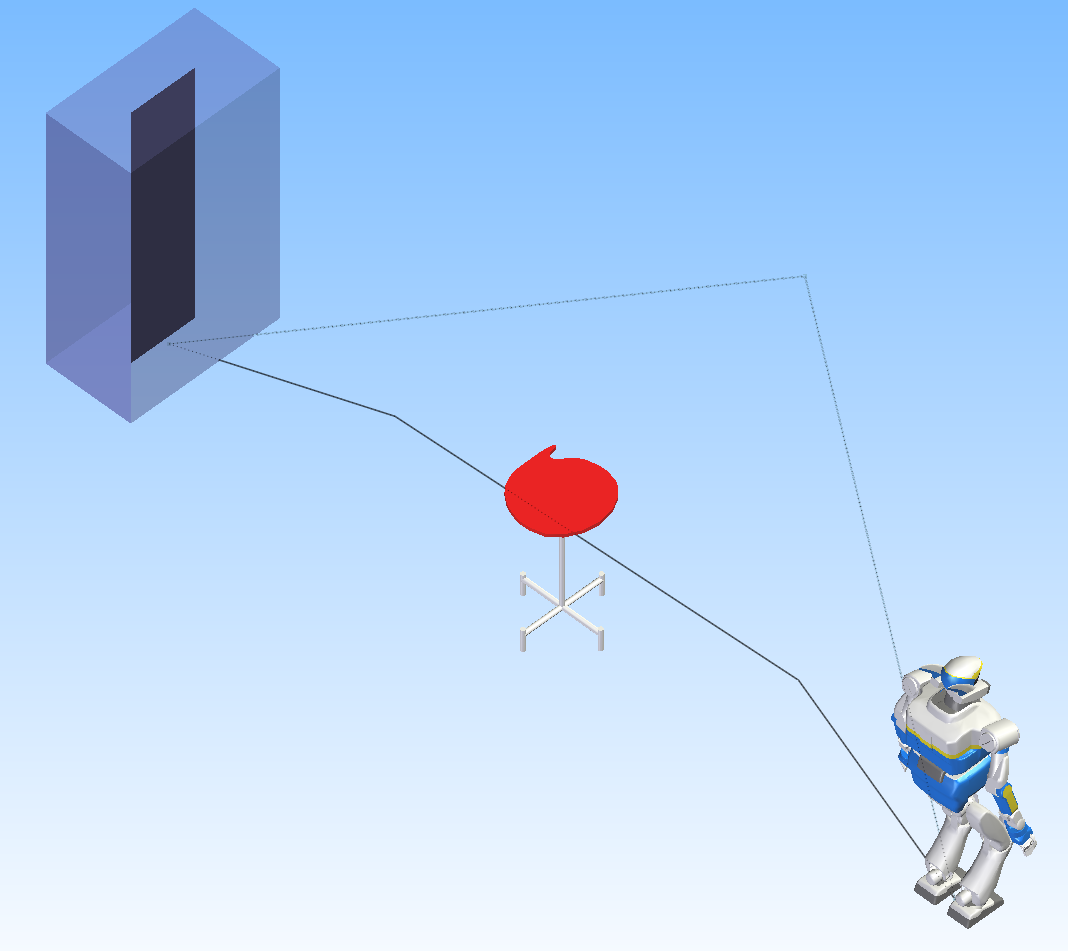
\includegraphics[height=.33\paperheight]{%
      src/chap1-roboptim/straight-line-obstacle.png}
    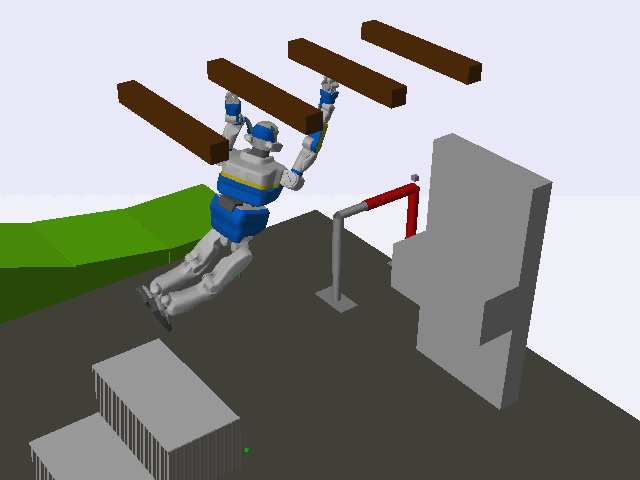
\includegraphics[height=.33\paperheight]{%
      src/slides/agent-067.jpg}\par
    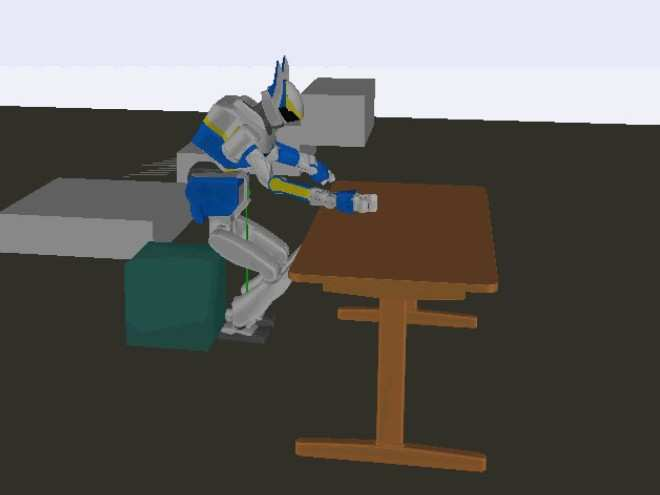
\includegraphics[height=.33\paperheight]{%
      src/slides/multi-014.jpg}
    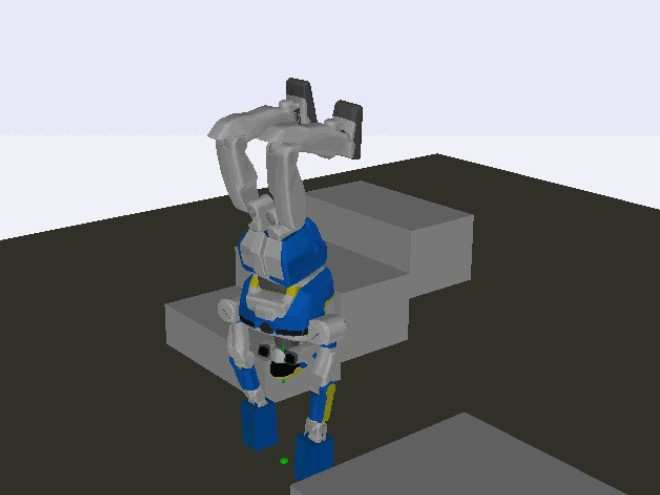
\includegraphics[height=.33\paperheight]{%
      src/slides/multi-015.jpg}

    Figures 2, 3, 4: K. Bouyarmane et collab.
  \end{center}
\end{slideDecision}

\fullFrameVideo{src/slides/multi-014.jpg}{vid/karim-multi-contact.mp4}{}


%%%%%%%%%%%%%%%%%%%%%%%%%%
\againframe<8>{contrib}

\begin{slideDecision}
  \frametitle{Génération de mouvements}

  \note[item]{Contraintes = plus de temps de calcul ainsi
  que possiblement plus de minima locaux.}
  \note[item]{Exemple: contrainte de distances/évitement d'obstacles.}
  \note[item]{Travail effectué: représentation du problème pour
    trouver équilibre entre réalisme, sûreté et tractabilité.}

  \begin{changeleftmargin}{1.1cm}
  \begin{center}
    Quelles contraintes?\par
    \vspace{1cm}
    
\includegraphics[width=.25\paperheight]{src/slides/falling.pdf}%
    
\includegraphics[width=.25\paperheight]{src/slides/burning.pdf}\par
  \end{center}

  \begin{itemize}
  \item Limites en position, vitesse et couple,
  \item (auto-)collision,
  \item \alert{équilibre}.
  \end{itemize}
  \end{changeleftmargin}
\end{slideDecision}

\begin{slideDecision}
  \frametitle{Équilibre (1)}

  \begin{changeleftmargin}{1.1cm}
    \begin{center}
      \vspace{-1cm}
      \begin{tikzpicture}[%
          force/.style={>=latex,
            draw=Thoughtless,
            fill=Thoughtless,
            ultra thick},
        ]
        \node (body) {
\includegraphics[height=6cm]{%
            src/slides/walking.pdf}};

        % Floor
        \draw[ultra thick] ([yshift=5]body.south west)
        -- ([yshift=5]body.south east);

        % Center of mass.
        \fill[radius=0.4em] ([xshift=-5.5]body.center) -- ++(0.4,0)%
        arc [start angle=0,end angle=90] -- ++(0,-0.4)%
        arc [start angle=270, end angle=180];%
        \draw[radius=0.4em] (body.center) circle;%

        % Forces
        \draw[force,->] (body.center)
        -- ++(0,-1) node[left] {$\mathcal{P}$};

        \draw[force,->] ([xshift=-15,yshift=5]body.south east)
        -- ++(0,1) node[right] {$f_c$};
      \end{tikzpicture}

      \begin{columns}
        \begin{column}{.5\paperwidth}
          \begin{equation*}
            \mathbf{x} = (\dot{x_G}, \dot{y_G}, \dot{z_G})
          \end{equation*}
        \end{column}
        \begin{column}{.5\paperwidth}
          \begin{equation*}
            \left(
            \begin{array}{c}
              \dot{\mathbf{x}}\\
              \dot{\sigma}
            \end{array}
            \right) = f(m, f_c)
          \end{equation*}
        \end{column}
      \end{columns}
    \end{center}
  \end{changeleftmargin}
\end{slideDecision}


\begin{slideDecision}
  \frametitle{Équilibre (2)}

  \note[item]{Critère de stabilité.}
  \note[item]{Point virtuel.}

  \begin{changeleftmargin}{1.1cm}
    \begin{center}
      ZMP dans le polygone support: mouvement
      dynamiquement stable.

      \bigskip

      \begin{tikzpicture}[%
          auto,
          footprint/.style={%
            rectangle,
            draw=black,
            ultra thick,
            minimum size=6mm,
            text width=8mm,
            decoration={brace},
        },
        fpLeft/.style={%
          footprint,
          decoration={brace, raise=-1.05cm},
        },
        fpRight/.style={%
          footprint,
          decoration={brace, raise=1.05cm},
        },
        supportPolygon/.style={%
          draw,
          ultra thick
        },
        zmpPoint/.style={%
          fill=ThoughfulBrick,
        }]

        \matrix[ampersand replacement=\&,
          row sep=1cm, column sep=.5cm]{%
            \uncover<1-6> {
              \node[fpLeft] (l0) {};
            } \&
            \&
            \uncover<8-> {
              \node[fpLeft] (l1) {};
            }\\
%
            \uncover<1-2> {
              \node[fpRight] (r0) {};
            }\&
            \uncover<4-10> {
              \node[fpRight] (r1) {};
            } \&
            \&
            \uncover<12-> {
              \node[fpRight] (r2) {};
            }\\
          };

        \uncover<1>{
          \draw[zmpPoint] (barycentric cs:l0=1/2,r0=1/2) circle (1mm);
        }
        \uncover<2-4>{
          \draw[zmpPoint] (l0) circle (1mm);
        }
        \uncover<5>{
          \draw[zmpPoint] (barycentric cs:l0=1/2,r1=1/2) circle (1mm);
        }
        \uncover<6-8>{
          \draw[zmpPoint] (r1) circle (1mm);
        }
        \uncover<9>{
          \draw[zmpPoint] (barycentric cs:l1=1/2,r1=1/2) circle (1mm);
        }
        \uncover<10-12>{
          \draw[zmpPoint] (l1) circle (1mm);
        }
        \uncover<13>{
          \draw[zmpPoint] (barycentric cs:l1=1/2,r2=1/2) circle (1mm);
        }
        \uncover<14>{
          \draw[zmpPoint] (r2) circle (1mm);
        }


        % 1/ double support.
        \uncover<1-2> {
          \path[supportPolygon]
          (l0.north west) -- (r0.south west)
          -- (r0.south east) -- (l0.north east) -- cycle;
          }

        % 2/ single support, left
        \uncover<3> {
          \path[supportPolygon]
          (l0.north west) -- (l0.south west)
          -- (l0.south east) -- (l0.north east) -- cycle;
        }

        % 3/ double support lr
        \uncover<4-6> {
          \path[supportPolygon]
          (l0.north west) -- (l0.north east)
          -- (r1.north east) -- (r1.south east) -- (r1.south west)
          -- (l0.south west) -- cycle;
        }

        % 4/ single support, right
        \uncover<7> {
          \path[supportPolygon]
          (r1.north west) -- (r1.south west)
          -- (r1.south east) -- (r1.north east) -- cycle;
        }

        % 5/ double support rl
        \uncover<8-10> {
          \path[supportPolygon]
          (l1.north west) -- (l1.north east)
          -- (l1.south east)
          -- (r1.south east) -- (r1.south west)
          -- (r1.north west) -- (l1.north west)
          -- cycle;
        }

        % 6/ single support, left
        \uncover<11> {
          \path[supportPolygon]
          (l1.north west) -- (l1.south west)
          -- (l1.south east) -- (l1.north east) -- cycle;
        }

        % 3/ double support lr
        \uncover<12-14> {
          \path[supportPolygon]
          (l1.north west) -- (l1.north east);
          \path[supportPolygon]
          (l1.north west) -- (l1.south west);


          \path[supportPolygon]
          (r2.south west) -- (r2.south east);
          \path[supportPolygon]
          (r2.south east) -- (r2.north east);

          \path[supportPolygon]
          (l1.south west) -- (r2.south west);
          \path[supportPolygon]
          (l1.north east) -- (r2.north east);
        }
      \end{tikzpicture}

    \end{center}
  \end{changeleftmargin}
\end{slideDecision}

\begin{slideDecision}
  \frametitle{Équilibre (3)}

  \note[item]{La position du ZMP évolue
    en fonction de la position/accélération du CoM
    ainsi que de la dérivée du moment cinétique.}
  \note[item]{On veut l'inverse: spécificer la trajectoire du ZMP et
    en déduire la trajectoire de CoM.}
  \note[item]{En temps réel! Ici pas le cas.}

  \begin{changeleftmargin}{1.1cm}
  \begin{center}
    \only<1-2>{%
      \begin{equation*}
        \begin{array}{lll}
          x_{ZMP} &=& x_G -
          \frac{\tikz \node[mathbox,%
              onslide=<2->{cross out,draw=ThoughfulBrick}]{$\dot{\sigma}_y$};
            + m z_G \ddot{x}_G}{%
            m (\tikz \node[mathbox,%
              onslide=<2->{cross out,draw=ThoughfulBrick}] {$\ddot{z}_G$}; + g)}\\
          y_{ZMP} &=& y_G +
          \frac{\tikz \node[mathbox,%
              onslide=<2->{cross out,draw=ThoughfulBrick}] {$\dot{\sigma}_x$}; -
            m z_G \ddot{y}_G}{%
            m (\tikz \node[mathbox,%
              onslide=<2->{cross out,draw=ThoughfulBrick}] {$\ddot{z}_G$}; + g)}
        \end{array}
      \end{equation*}
    }
    \only<3>{%
      \begin{equation*}
        \begin{array}{lll}
          x_{ZMP} &=& x_G - \frac{z_G}{g} \ddot{x_G}\\
          y_{ZMP} &=& y_G - \frac{z_G}{g} \ddot{y_G}
        \end{array}
      \end{equation*}
    }
  \end{center}

  \begin{description}
    \item[$(x_G, y_G, z_G)$]~\\
      Position du centre de masse (CoM).
    \item[$(\sigma_x, \sigma_y)$]~\\
      Moment cinétique autour du centre de masse.
    \item[$m$] Masse du robot.
    \item[$g$] Constante de gravité.
  \end{description}

  \end{changeleftmargin}
\end{slideDecision}

\begin{slideDecision}
  \frametitle{Génération de mouvements}

  \note[item]{Détailler les étapes.}
  \note[item]{Trajectoire corps complet dans la planif: pas de
    comportement réactif.}

  \begin{changeleftmargin}{1.5cm}
  \begin{center}
    \begin{enumerate}
      \item Génération d'une pile de pas.
      \item Génération d'une trajectoire de ZMP.
      \item Génération de la trajectoire de centre de masse
        correspondante.
      \item Génération des trajectoires de pieds.
    \end{enumerate}

    \bigskip

    \alert{Et la trajectoire corps complet?}
  \end{center}
  \end{changeleftmargin}
\end{slideDecision}

\maxFrameImageWidth{src/chap3-primitive-mouvement/footsteps1.jpg}

\begin{slideAction}
  \frametitle{Contrôleur polyvalent (2)}

  \note[item]{Deux types de tâches. Point6D et CoM.}
  \note[item]{Peut également ajouter butées, vitesse
    maximum mais pas d'inégalités en pratique.}
  \note[item]{Ici tâches ``de base'' mais on peut également
    ajouter des tâches de priorité moindre: tête.}
  \note[item]{Il manque le rebouclage capteur. Comment faire?}

  \begin{changeleftmargin}{1.1cm}
  \begin{center}

    \begin{tikzpicture}[%
        >=latex,
        node distance=1em,
        fixed/.style={
          text width=120pt}]
      \node [state,fixed] (com) {Centre de masse};
      \node [state,fixed, below=of com] (lf) {Pied gauche};
      \node [state,fixed, below=of lf] (rf) {Pied droit};
      \node [state,fixed, below=of rf] (posture) {Posture};

      \node [left=of com] (fort) {Priorité forte};
      \node [left=of posture] (faible) {Priorité faible};
      \draw[->, line width=1.05]
      (fort.south) -- (faible.north);
    \end{tikzpicture}
  \end{center}
  \end{changeleftmargin}
\end{slideAction}

\fullFrameVideo{src/slides/over.jpg}{vid/humanoids11-lbaudouin3.mp4}{%
    \tiny{%
      \vspace{-.6cm}%
      ~
\includegraphics[height=.25cm]{src/slides/idea.pdf}~%
      Real-time Replanning Using 3D Environment for Humanoid Robot,
      Proc. of Humanoids'11.%
    }%
}

\begin{slideAction}
  \frametitle{Motivation}

  \note[item]{FIXME: expliquer le code couleur des pieds}
  \note[item]{Pourquoi y a-t-il une dérive après la correction?}


  \begin{center}
    \begin{tikzpicture}[>=latex]
        \def\w{0.5}
        \def\h{0.75}

        \foreach \dy in {0., 1., 2., 3.}
                 {
                   % left step planned
                   \filldraw[pattern=north east lines] (0., \dy)
                   rectangle (0. + \w, \dy + \h);

                   % right step planned
                   \filldraw[pattern=north west lines] (1., \dy + 0.5)
                   rectangle (1. + \w, \dy + \h + 0.5);
                 }

        % before correction
        \def\driftx{0.1}
        \def\drifty{0.05}
        \def\drifttheta{5.}

        \def\dy{0}
        % left step planned
        \draw<2->[style=solid, color=red, rotate=\drifttheta * \dy,line width=1.25]
        (0. + \driftx * \dy, \drifty * \dy + \dy)
        rectangle (0. + \driftx * \dy + \w, \drifty * \dy + \dy + \h);

        % right step planned
        \draw<3->[style=solid, color=red, rotate=\drifttheta * \dy + \drifttheta / 2.,line width=1.25]
        (1. + \driftx * \dy + \drifty / 2., \drifty * \dy + \drifty / 2. + \dy + 0.5)
        rectangle (1. + \driftx * \dy + \drifty / 2. + \w, \drifty * \dy + \drifty / 2. + \dy + \h + 0.5);

        \def\dy{1}
        % left step planned
        \draw<4->[style=solid, color=red, rotate=\drifttheta * \dy,line width=1.25]
        (0. + \driftx * \dy, \drifty * \dy + \dy)
        rectangle (0. + \driftx * \dy + \w, \drifty * \dy + \dy + \h);

        % right step planned
        \draw<5->[style=solid, color=red, rotate=\drifttheta * \dy + \drifttheta / 2.,line width=1.25]
        (1. + \driftx * \dy + \drifty / 2., \drifty * \dy + \drifty / 2. + \dy + 0.5)
        rectangle (1. + \driftx * \dy + \drifty / 2. + \w, \drifty * \dy + \drifty / 2. + \dy + \h + 0.5);


        \def\dy{2}
        \draw<6->[style=solid, color=red,line width=1.25, rotate=\drifttheta] (0. + \driftx, \dy + \drifty)
        rectangle (0. + \w + \driftx, \dy + \h + \drifty);

        % --- after correction ---

        % left step planned
        \draw<7->[style=solid, color=green,line width=1.25] (0., \dy)
        rectangle (0. + \w, \dy + \h);

        \uncover<7->{
        \draw[smooth,rounded corners=1ex,<-,thick]
        (-0.3, \dy) -- (-0.3 - 0.05, \dy + 0.2) -- (-0.3 - 0.2, \dy + 0.4)
        node[midway,left]
        {
          $\delta \mathbf{x}$
        };
        }


        \draw<7->[style=solid, color=green,line width=1.25] (0., \dy)
        rectangle (0. + \w, \dy + \h);
        \draw<7->[style=solid, color=green,line width=1.25] (1., \dy + 0.5)
        rectangle (1. + \w, \dy + \h + 0.5);
        \def\dy{3}
        \draw<7->[style=solid, color=green,line width=1.25] (0., \dy)
        rectangle (0. + \w, \dy + \h);
        \draw<7->[style=solid, color=green,line width=1.25] (1., \dy + 0.5)
        rectangle (1. + \w, \dy + \h + 0.5);

        % right step planned
        \def\dy{2}
        \draw<8->[style=solid, color=orange,line width=1.25, rotate=\drifttheta * 0.5] (1. + \driftx * .5, \dy + 0.5 + \drifty * 0.5)
        rectangle (1. + \driftx * 0.5 + \w, \dy + \drifty * 0.5 + \h + 0.5);

        \def\dy{3}
        % left step planned
        \draw<9->[style=solid, color=orange,line width=1.25, rotate=\drifttheta * 1.] (0. + \driftx * 1., \dy + \drifty * 1.)
        rectangle (0. + \w + \driftx * 1., \dy + \h + \drifty * 1.);

        % right step planned
        \uncover<10-> {
          \draw[style=solid, color=orange,line width=1.25, rotate=\drifttheta * 1.5] (1. + \driftx * 1.5, \dy + 0.5 + \drifty * 1.5)
        rectangle (1. + \w + \driftx * 1.5, \dy + \h + 0.5 + \drifty * 1.5);
        }

      \end{tikzpicture}
      \end{center}
\end{slideAction}


\begin{slideAction}
  \frametitle{Contrôleur temps réel}

  \note[item]{Actionement: nécessité d'envoyer une commande
    à une période fixe. Contraint le temps de calcul.}

  \begin{changeleftmargin}{1.1cm}
  \begin{center}
    Contrôleur: algorithme générant la commande envoyée aux moteurs à
    une fréquence fixe (200Hz pour HRP-2).

    \bigskip

    \begin{itemize}
    \item Exécute les tâches générées par la partie décisionelle.
    \item Permets l'adaptation réactive du mouvement.
    \end{itemize}

    \bigskip

    Composant \alert{critique} de tout robot.
  \end{center}
  \end{changeleftmargin}
\end{slideAction}


\begin{slideAction}
  \frametitle{Schéma de contrôle}

  \note[item]{Ajout du rebouclage capteur en déformant
  les références des tâches.}
  \note[item]{Localisation externe.}
  \note[item]{Intérêt du fonctionnement par tâche.}

  \begin{changeleftmargin}{1.1cm}
  \begin{center}
    \begin{tikzpicture}[%
        >=latex]
      \node[state] (gen) {Génération};
      \node[state, below=of gen] (corr) {Correction};
      \node[state, below=of corr, align=left,inner sep=0.1ex,
        shape=rectangle split,
        rectangle split part align=left,
        rectangle split parts=5] (ctrl) {Contrôleur%
        \nodepart{two}\footnotesize{centre de masse}
        \nodepart{three}\footnotesize{pied gauche}
        \nodepart{four}\footnotesize{pied droit}
        \nodepart{five}\footnotesize{posture}};
      \node[state,right=2cm of corr] (loc) {Localisation};

      %\draw[-,style=dashed] (2,-3) -- (2,3);

      \uncover<3-> {
        \draw[->] (loc.west) -- (corr.east)
        node [at start,left,font=\tiny,yshift=0.2cm]
        {$\hat{\mathbf{x}}_t$};
      }

      \uncover<2-> {
        \draw[->] (gen.south) -- (corr.north)
        node [at start,right,font=\tiny,yshift=-0.2cm]
        {$(\gamma_{\text{pieds}}(t), \gamma_{\text{com}}(t))$};
      }

      \uncover<3-> {
        \draw[->] (corr.south) -- (ctrl.north)
        node [at start,right,font=\tiny,yshift=-0.25cm]
        {$(\gamma'_{\text{pieds}(t)}, \gamma'_{\text{com}}(t))$};
      }

      \uncover<4-> {
        \draw[->] (ctrl.south) --++ (0,-1)
        node [at start,right,font=\tiny,yshift=-0.25cm]
        {$\dot{\mathbf{q}}_t$};
      }

      \draw[<-] (gen.north) --++ (0,1) node [left,font=\tiny,yshift=-0.25cm]
           {$\mathbf{S}$};
    \end{tikzpicture}%
    %
    \footnotesize{%
      \hspace{-5cm}%
      
\includegraphics[height=.5cm]{src/slides/idea.pdf}~%
      Trajectory Following for Legged Robots, Proc. of Biorob'12.%
    }%
  \end{center}
  \end{changeleftmargin}
\end{slideAction}

\begin{slideAction}
  \frametitle{Synchronisation temporelle}

  \begin{center}
    \vspace{-.5cm}
    \begin{tikzpicture}
      \begin{axis}[
          grid=major,
          legend style={
            at={(0.5,-0.2)},
            anchor=north,
            legend columns=3,
            cells={anchor=west},
            font=\footnotesize,
            rounded corners=2pt,
            draw=white
          },
          xlabel=time ($s$),
          ylabel=$x$ position ($m$),
          no markers,
          yticklabel pos=lower
          ]

        \addplot[
          Thoughtless, thick,
          dashed
        ] table [
          x expr=(\thisrowno{0}-0)*0.005,
          y expr=\thisrowno{1}+0.04
          ]{dat/feet_follower_feet-follower-com.dat};
        \addlegendentry{centre de masse}

        \addplot[
          ThoughtYouWere,
          dashed,
        ] table[
          x index=0,
          y index=4,
          x expr=(\thisrowno{0}-0)*0.005,
          y expr=\thisrowno{4}+0.04
        ] {dat/feet_follower_feet-follower-left-ankle.dat};
        \addlegendentry{pied gauche}

        \addplot[
          Thoughtless2, thick,
          dashed,
        ] table[
          x index=0,
          y index=4,
          x expr=(\thisrowno{0}-0)*0.005,
          y expr=\thisrowno{4}+0.04
        ] {dat/feet_follower_feet-follower-right-ankle.dat};
        \addlegendentry{pied droit}

        \addplot[
          Thoughtless, thick,
        ] table[
          x expr=(\thisrowno{0}-0)*0.005
        ]{dat/feet_follower_correction-com.dat};
        \addlegendentry{centre de masse (corr.)}

        \addplot[
          ThoughtYouWere, thick,
        ] table[
          x index=0,
          y index=4,
          x expr=(\thisrowno{0}-0)*0.005,
        ] {dat/feet_follower_correction-left-ankle.dat};
        \addlegendentry{pied gauche (corr.)}

        \addplot[
          Thoughtless2, thick,
        ] table[
          x index=0,
          y index=4,
          x expr=(\thisrowno{0}-0)*0.005,
        ] {dat/feet_follower_correction-right-ankle.dat};
        \addlegendentry{pied droit (corr.)}
      \end{axis}

      \def\w{0.5}
      \def\h{0.75}
      \def\dx{8.}

      \def\dy{.5}
      % left step planned 1
      \filldraw[pattern=north east lines,%
        draw=ThoughtYouWere] (\dx + 0., \dy + 0.5)
      rectangle (\dx + 0. + \w, \dy + \h + 0.5);

      % left step planned 1 - drift
      \uncover<2-> {
        \draw[style=solid,draw=ThoughtYouWere,%
          line width=1.25] (\dx, \dy - 0.3 + 0.5)
        rectangle (\dx + \w, \dy + \h - 0.3 + 0.5);
      }

      \filldraw[pattern=north east lines,%
        draw=Thoughtless2] (\dx + 1., \dy + 0.5)
      rectangle (\dx + 1. + \w, \dy + \h + 0.5);
      \draw<2->[style=solid,color=Thoughtless2,%
        line width=1.25] (\dx + 1., \dy - 0.3 + 0.5)
      rectangle (\dx + \w + 1., \dy + \h - 0.3 + 0.5);


      % right step planned 1
      \filldraw[pattern=north east lines,%
        draw=Thoughtless2] (\dx + 1., \dy + 3.)
      rectangle (\dx + 1. + \w, \dy + \h + 3.)
      node [pos=0.5,anchor=north,font=\tiny,yshift=0.75cm] {pas 1};

      % right step planned 1 - corrected
      \uncover<2-> {
        \draw[style=solid,draw=Thoughtless2,line width=1.25]
        (\dx + 1., \dy + 3.-0.3)
        rectangle (\dx + 1. + \w, \dy + \h + 3. -0.3);
      }

      \uncover<3-> {
        \draw[style=solid,draw=Thoughtless2,%
          line width=1.25] (\dx + 1., \dy + 3.)
        rectangle (\dx + 1. + \w, \dy + \h + 3.);
      }

      \def\dy{3.}
      % left step planned 2
      \filldraw[pattern=north east lines,%
        draw=ThoughtYouWere] (\dx + 0., \dy + 0.5)
      rectangle (\dx + 0. + \w, \dy + \h + 0.5)
      node [pos=0.5,anchor=north,font=\tiny,yshift=0.75cm] {pas 2};

      \uncover<2-> {
        \draw[style=solid,draw=ThoughtYouWere,%
          line width=1.25] (\dx, \dy + 0.5 -0.3)
        rectangle (\dx + \w, \dy + \h + 0.5 -0.3);
      }

      % left step planned 2 - corrected
      \uncover<4-> {
        \draw[style=solid,draw=ThoughtYouWere,%
          line width=1.25] (\dx + 0., \dy + 0.5)
      rectangle (\dx + 0. + \w, \dy + \h + 0.5);
      }
    \end{tikzpicture}
  \end{center}
\end{slideAction}

\begin{slideAction}
  \frametitle{Trajectoire du centre de masse}

  \note[item]{Préservation de la stabilité.}
  \note[item]{Opérateur linéaire.}
  \note[item]{Ici delta $E^2$.}

  \begin{equation*}
    \mathbf{z} = \mathbf{c} - \frac{z_c}{g} \ddot{\mathbf{c}}
  \end{equation*}

  \begin{equation*}
    \mathbf{c}^{(n)}(t) =
    \underbrace{\scriptstyle \cosh(\sqrt{\frac{g}{z_c}}.t) . \mathbf{V} +
      \sinh(\sqrt{\frac{g}{z_c}}.t) . \mathbf{W} +
      \mathbf{r}(t)}_{\mathbf{c}(t) \in \mathbb{R}^2} + \sum_{i=1}^n \Delta^{t_i}(t)
  \end{equation*}

  \begin{center}
    $\mathbf{V}$, $\mathbf{W}$ déterminent la position et vitesse
    initiale.
  \end{center}

  \begin{equation*}
    \forall t \in \mathbb{R}, \Delta^t(0) = \dot{\Delta}^t(0) = 0
  \end{equation*}
\end{slideAction}

\fullFrameVideo{src/slides/demo.jpg}{vid/biorob12.mp4}{}

%%%%%%%%%%%%%%%%%%%%%%%%%%
\againframe<9>{contrib}

\fullFrameVideo{src/slides/door.jpg}{vid/hrp2-opening-door.mp4}{}

\begin{slideAction}
  \frametitle{Primitives de mouvement}

  \note[item]{Nécessaire d'adapter la pile de tâches
    à l'opération en cours. Dépend du scénario.}
  \note[item]{La localisation également diffère selon
    les cas.}
  \note[item]{La localisation globale parfaite d'un robot est
    difficile mais surtout souvent inutile. L'erreur de localisation
    doit décroître avec l'acomplissement de la tâche.}
  \note[item]{Il est nécessaire de planifier les tâches et
    l'asservissement de façon jointe.}
  \note[item]{Actuellement planification corps complet puis extraction
    des tâches. Choix de l'asservissement manuel.}


  \begin{changeleftmargin}{1.1cm}
  \begin{center}
    \begin{tikzpicture}[%
        node distance=1em,
        inner sep=0.1ex,
        outer sep=0.1ex,
        fixed/.style={
          text width=40pt}]

      \matrix[ampersand replacement=\&,
        row sep=.5cm, column sep=.5cm]{%
        \node {%
          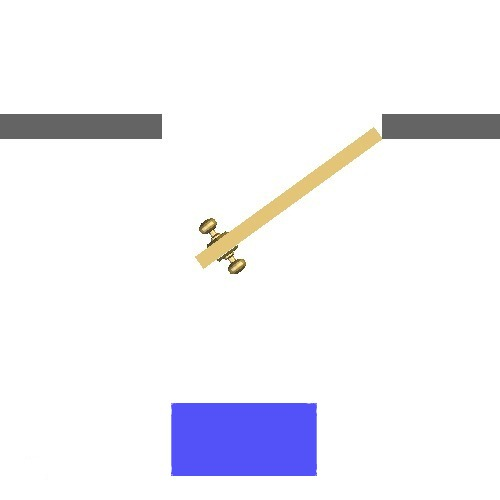
\includegraphics[height=1.5cm]{src/slides/doorstate1.jpg}};\&
        \node {%
          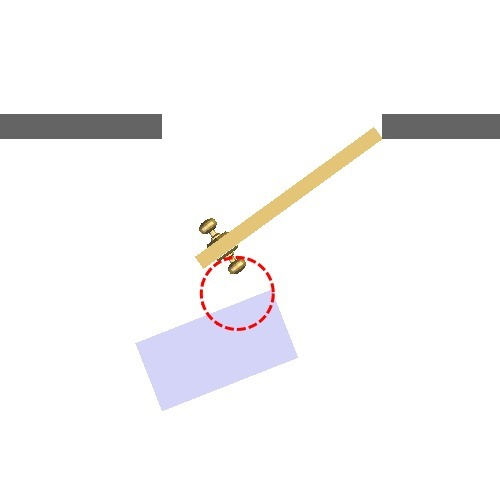
\includegraphics[height=1.5cm]{src/slides/doorstate2.jpg}};\&
        \node {%
          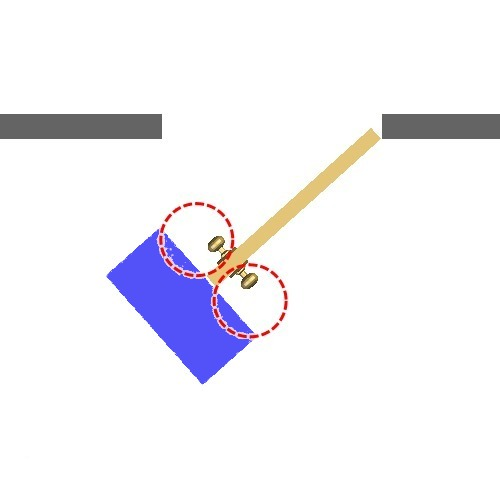
\includegraphics[height=1.5cm]{src/slides/doorstate3.jpg}};\&
        \node {%
          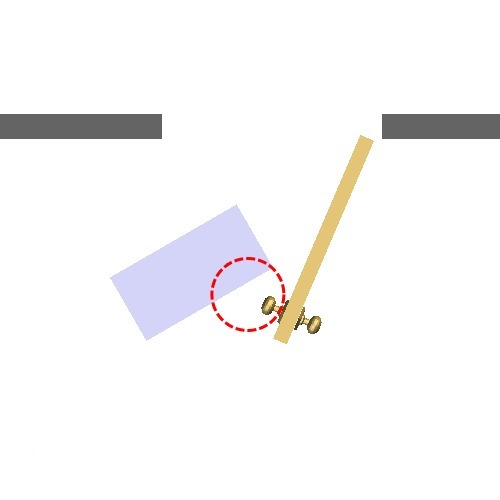
\includegraphics[height=1.5cm]{src/slides/doorstate4.jpg}};\\
        \node[state,fixed] {\tiny{Équilibre}};\&
        \node[state,fixed] {\tiny{Équilibre}};\&
        \node[state,fixed] {\tiny{Équilibre}};\&
        \node[state,fixed] {\tiny{Équilibre}};\\
%
        \node [state,fixed] {\tiny{Posture}};\&
        \node [state,fixed] {\tiny{Bras droit}};\&
        \node [state,fixed] {\tiny{Bras gauche}};\&
        \node [state,fixed] {\tiny{Bras gauche}};\\
%
        \&
        \node [state,fixed] {\tiny{Posture}};\&
        \node [state,fixed] {\tiny{Bras droit}};\&
        \node [state,fixed] {\tiny{Posture}};\\
%
        \&
        \&
        \node [state,fixed] {\tiny{Posture}};\&
        \\

        \node[state,fixed,color=ThoughtBySome,fill=Thoughtless2]
             {\tiny{Porte}};\&
        \node[state,fixed,color=ThoughtBySome,fill=Thoughtless2]
             {\tiny{Poignée}};\&
        \node[state,fixed,color=ThoughtBySome,fill=Thoughtless2]
             {\tiny{Poignée}};\&
        \node[state,fixed,color=ThoughtBySome,fill=Thoughtless2]
             {\tiny{Poignée}};\\
      };
    \end{tikzpicture}
  \end{center}
  \end{changeleftmargin}
  \vbox{%
    \tikz \node[state,
      color=ThoughtBySome,fill=Thoughtless2] {\tiny{Asservissement}};
    \tikz \node[state] {\tiny{Tâche}};
  }
\end{slideAction}

%%%%%%%%%%%%%%%%%%%%%%%%%%
\againframe<10>{contrib}

\begin{slidePerception}
  \frametitle{Systèmes de localisation}

  \note[item]{Parler d'intégration logicielle.  Mentioner ROS
    rapidement.}

  \begin{changeleftmargin}{1.1cm}
  \begin{description}
  \item[Capture de mouvement]~\\
    Précision $\pm 1$ cm. Environnement instrumenté.
  \item[Suivi d'objet]~\\
    Précision à quelques centimètres près. Méthode locale.
  \item[Odométrie visuelle]~\\
    Précision plus faible. Méthode globale.
  \end{description}
  \end{changeleftmargin}
\end{slidePerception}

\maxFrameImageHeight{src/chap4-integration/shelf.png}

\begin{slidePerception}
  \frametitle{Contributions logicielles (1)}

  \begin{changeleftmargin}{1.1cm}
    \begin{itemize}
      \item Interface Python pour le contrôle robotique.
      \item Module Python pour la manipulation de modèles de robots.
      \item Interfaces pour la représentation des problèmes de marche.
      \item Formalisation de la représentation des robots humanoïdes.
      \item Intégration d'un algorithme de suivi dans un composant
        ROS, du système de capture de mouvement.
      \item Participation au portage du modèle des robots HRP-2 et
        Romeo en URDF.
    \end{itemize}
  \end{changeleftmargin}
\end{slidePerception}

\begin{slidePerception}
  \frametitle{Contributions logicielles (2)}

  \begin{changeleftmargin}{1.1cm}
    \begin{itemize}
      \item Portage de l'architecture complète du robot HRP-2 sous
        ROS: contrôle, capteurs (IMU, vision), planification.
      \item Amélioration des bibliothèques bas-niveau et de
        l'architecture logicielles du planificateur de pas (HPP).
      \item C++: \~ 100k lignes modifiées / Python: \~ 5k lignes
        modifiées (source: Ohloh.net).
    \end{itemize}

    \bigskip

    
\includegraphics[height=.5cm]{src/slides/idea.pdf}~%
    Coordinate Frames for Humanoid Robots, REP 120.

  \end{changeleftmargin}
\end{slidePerception}

\maxFrameImageHeight{src/chap3-primitive-mouvement/calibextrinsic.jpg}

\begin{frame}
  \frametitle{Conclusion}

  \note[item]{Polyvalence.}
  \note[item]{Intégration.}
  \note[item]{Scénarii complexes pour étendre les capacités des robots
    humanoïdes.}
  \note[item]{Faire le lien entre la planification et l'exécution.}
  \note[item]{Démontre le fossé entre robotique et simulation
    robotique.}

  \begin{itemize}
  \item Architecture complète: perception, décision, action.
  \item Correction des pas pour les mouvements de précision.
  \end{itemize}

  \bigskip

  \begin{itemize}
  \item Valider l'approche pour les bras.
  \item Valider les pas corrigés en ligne.
  \item Améliorer la localisation du robot. Utilisation conjointe de
    plusieurs systèmes de localisation.
  \end{itemize}
\end{frame}

\maxFrameImage{src/slides/hrp2-thx.jpg}


%
%\begin{slidePerception}
%  \frametitle{De la bibliothèque au composant}
%
%  FIXME
%\end{slidePerception}

%\maxFrameImageHeight{src/slides/demo2.jpg}

%\maxFrameImageHeight{src/chap4-integration/footsteps2.jpg}
%\maxFrameImageHeight{src/chap4-integration/disparity-1.jpg}
%\maxFrameImageHeight{src/chap4-integration/disparity-2.jpg}
%\maxFrameImageHeight{src/chap4-integration/hrp2_urdf.jpg}
%\maxFrameImageHeight{src/chap4-integration/rviz-full.jpg}



\end{document}
